\begin{figure}[t]
  \centering
  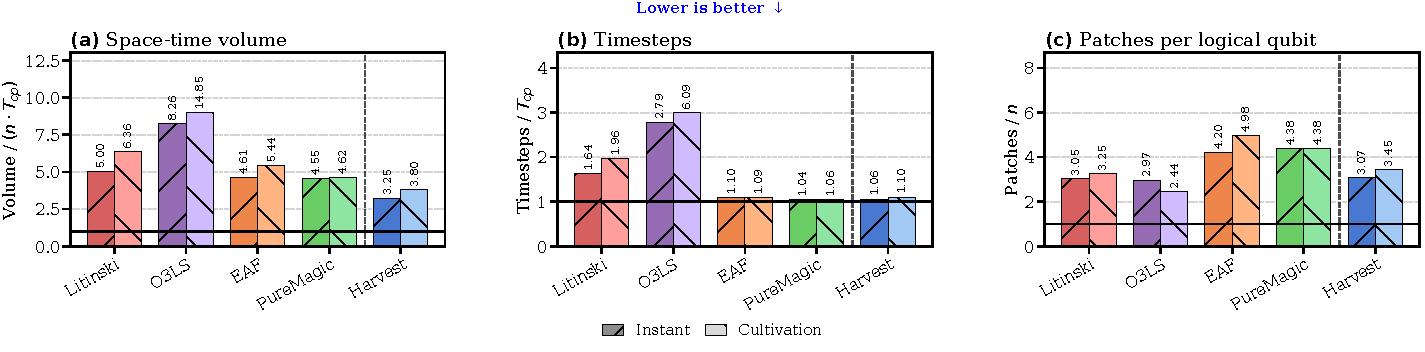
\includegraphics[width=\linewidth]{figures/evaluation/fig_rq1_sota.pdf}
  \caption{\textbf{Comparison with the state of the art} (RQ1). Geometric means over all circuits under instant (dark) and cultivated (light) magic states, normalized to circuit size $n$ and critical-path length $T_{cp}$. \textbf{(a)}~Space--time volume per data patch and critical-path step. \textbf{(b)}~Timesteps over the critical path. \textbf{(c)}~Patches per logical qubit. The solid line marks the respective lower bound: $n$ data patches for $T_{cp}$ steps. Bars above the axis limit are clipped and labeled with their value.}
  \label{fig:rq1-sota}
\end{figure}
